\subsubsection{Kubernetes} \label{sec:Kubernetes}
Kubernetes is the de-facto standard for container orchestration and the main technology used in this thesis. It is a highly complex tool and offers many  configurations, thus understanding the fundamentals is highly important. A deep understanding of Kubernetes resources also helps in understanding the current shortcoming concerning the edge. Kubernetes was designed from the ground up to be extensible, so the question is not if Kubernetes could do something, but rather if there is an existing implementation.

This section covers five important aspects of Kubernetes. First, single-cluster vs multi-cluster. Second, the core components of Kubernetes, mainly the kubelet, together with other resource configurations. Third, the optimal deployment strategy, how to control and secure resources and how to select nodes. Fourth,  how to do load balancing and, finally, how to do traffic control and shaping.\\[5mm]
% \vspace{0.5mm} \ \\
\textbf{\textit{Single vs. Multi-Cluster}}\\
% \subsubsection{Single vs. Multi-Cluster} \label{sec:singleVsMultiCluster}
Single cluster Kubernetes provides many techniques to isolate and allocate resources. It is recommended for all but very big or multi-cloud deployments, but has limitations which could be especially crucial on the edge. The official Kubernetes distribution has a multi-cluster management tool called Kubernetes Cluster Federation (KubeFed)\cite{kubernetesFederation97:online}. It provides another layer of fault isolation and because of multiple ingresses it enables low latency and scalability across regions. But requires additional management on top of Kubernetes already complicated control plane and is thus important for big deployments with high system requirements, multi-cloud solutions and edge deployments.\\
Google recently revealed a new and much hyped product, Anthos\cite{TechnicalAnthosGoogle66:online}. Its a combination of many services, but most importantly it lets people easily manage multi cluster deployments. Google describes it as follow: ``Anthos is a modern application management platform that provides a consistent development and operations experience for cloud and on-prem environments''\cite{TechnicalAnthosGoogle66:online}. Google provides an installer for on-prem devices but once installed Google itself manages the cluster including updates and troubleshooting. Not only is it a multi-cluster solution, but it also integrates the clusters with the Istio service mesh, providing unified communication and communication logs, and additional tools to ease the management. Anthos represents an industry wide trend for multi-cluster and multi-cloud solutions but is closed source. Compared to Anthos, Kubefed lacks many of features for easier management and is still in alpha status and thus not recommended for use in production environments.\\



\comment{
These will not fade away and still be important. Finally, Docker's strong selling point of its cloud edge solution is its mirrored registry and neat features around it. It is possible though to setup a Docker Hub\footnote{The official Docker registry for images \url{https://hub.docker.com/}.} mirror for on-prem solutions. 


}


% \vspace{0.5mm} \ \\
\textbf{\textit{Core Components}}\\
% \subsubsection{Core Components}
Kubernetes is complex and resource intensive tool. However, much of the resource overhead stems from the control plane which only runs on master nodes. These nodes are not in the scope of this thesis and thus not explained in more detail. Worker nodes on the other hand are orchestrated and provide their state to the master. This is a lot less resource intensive and there are a few tricks to reduce the resource load even further. For a worker node to be part of a cluster it needs to run the following components: the \textit{kubelet}, \textit{kube-proxy} and a supported container runtime. How Kubernetes works in practice can be seen in \cref{fig:nodeComponents}\footnote{The \textit{cAdvisor} component is a health checking tool and not required.}.
\begin{figure}[h!]
    \centering
    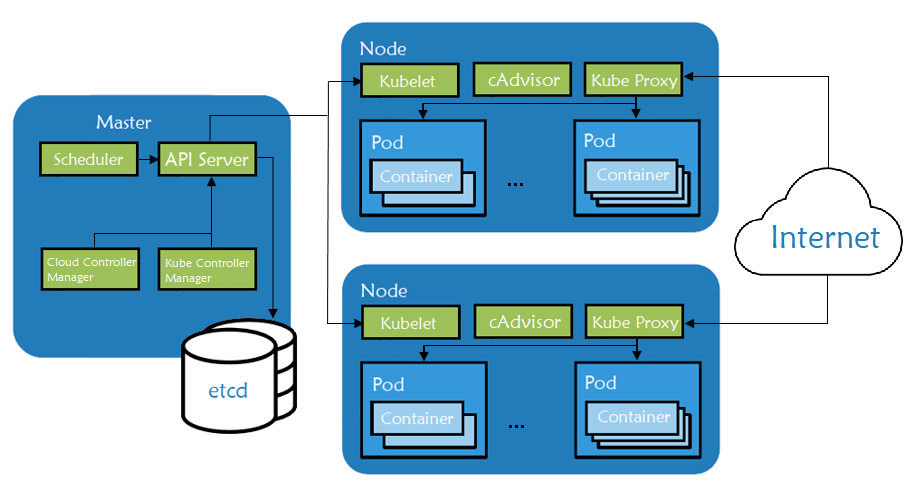
\includegraphics[scale=0.6]{figures/rancherK8sComponents.png}
    \caption{The Kubernetes Architecture and Node Components\cite{nodeSetupKubernetes:online}}
    \label{fig:nodeComponents}
\end{figure}
The kubelet is the primary node agent and schedules and maintains containers running inside a pod based on the pods \textit{PodSpecs}. It gets the these specifications mainly from the APIServer, but other Kubernetes internal sources are possible, too. Containers created outside of the cluster (or multi cluster) are not managed by the kubelet. 

Configuring the kubelet is easily possible via the kubectl and kubeadm tools which give the possibility of enhancing the kubelets performance for different circumstances, e.g. the edge. Going through the possible configurations under \url{https://kubernetes.io/docs/reference/command-line-tools-reference/kubelet/}, the most important configurations for the edge is the \textit{--housekeeping-interval duration} which defaults to 10s\cite{rancherKubernetesComponents:online}. This means each 10 seconds the kubelet performs a complete health check of all its components and sends it to the master. For normal cloud nodes this is a sensible choice. The nodes are powerful enough to handle the additional overhead and it avoids having unavailable resources. For light edge devices the interval is too high. The kubelet from k3s (discussed in \cref{sec:existingSolutions}) called hypervisor is compatible with vanilla Kubernetes and optimized for light edge devices.

For networking Kubernetes provides the kube-proxy which is a network proxy node agent ensuring that the Kubernetes networking services run on each node. It enables the Kubernetes service abstraction by ensuring the network rules on each host and carries out the connection forwarding. Kubernetes does not provide a standard implementation but requires the administrator to provide one at the installation. The last component, the container runtime (discussed in the \cref{sec:containers}), ensures that containers can run as expected.




% \vspace{0.5mm} \ \\
\textbf{\textit{Deployment Strategies}}\\
% \subsubsection{Deployment Strategies}
\comment{
deployment vs statefulset vs daemonset
clusterIP vs nodeport
Taints, nodeselector, affinities pod/node
namespaces
}
The \textit{service} resource provides an abstraction between the network interface and the actual application. From an outsiders view, it is possible to call the Kubernetes ingress gateway under a subsection and get to a pod running somewhere in the cluster without knowing its specific address. From the inside it enables routing between services based on the service name. Services are the usual deployment strategy for stateless applications. The pods are assigned a \textit{clusterIP} making it only accessible from inside the cluster, outside requests have to go through the cluster ingress and are then routed to a pod. This makes little sense on the edge, where latency is key and an Internet connection is not guaranteed. Instead, services offer the possiblity to define a \textit{nodePort} inside a service. It exposes a port from the pods to the host machine so that outside services can connect directly to the pod and the container listing for incoming connections.\\
Kubernetes also offers different resources for core workloads, \textit{Deployments},  \textit{StatefulSets},  \textit{DaemonSets} and  \textit{ReplicationController}, which should not be used anymore\cite{CoreWorkloadKubernetes66:online}. They all describe a desired state and the Kubernetes controller works towards fulfilling this desired state. Deployments are mainly used for stateless services. StatefulSets are used for stateful services and DaemonSets are to deploy pods on each node. For the edge all workloads are important, but it is important to choose the correct workload for a desired result. Inside the workloads specifications it is also possible to define resources. Because of the resource limitations of edge devices auto-scaling is not possible and devices can get quickly overwhelmed by too many tasks. This also puts an emphasis on the prioritization of workloads in case the hosts computing resources are not enough for all workloads.\\
Kubernetes offers powerful concepts to achieve the correct scheduling of pods on desired nodes. They are \textit{nodeSelector}, \textit{taints}, \textit{tollerations}, \textit{affinities} and \textit{anti-affinities}. A NodeSelector specifies which tags have to be present on a node for a pod to be scheduled on. Taints are added to nodes and specifies that only pods with the matching tolleration can run on the node. For exmaple, the master has the taint \textit{NoSchedule} which means, only pods with the matching tolleration can be scheduled on a the master. Finally, affinities and anti-affinities, offer a way for pods to be scheduled (or not) on either pods or nodes with a specific tag. This gives operators the ability to add workloads only on nodes which are already running another service, or with anit-affinity, where a pod is not present. Again, these are very powerful tools and have to be selected carefully.\\
Finally, \textit{namespaces} offer the ability to separate one physical cluster into mulitple virtual clusters. Most Kubernetes resources are saved inside namespaces which are especially important in a single-cluster setup with multiple user groups. Administrators can define namespaces and assign them resource limits as well as nodes via the \textit{PodNodeSelector}. This makes it possible to assign each logical edge deployment a virtual cluster and developers can only modify resources within that namespace. It is also possible to define role-based access control (RBAC) to limit what a specific user or user group can modify inside a namespace. 

\\[5mm]
\textbf{\leftskip25mm\textit{Load Balancing}}\\
Load balancing in a distributed environment is difficult as the ingress node needs a complete network topology at any given moment in time. This is one of the reasons why Kubernetes refreshes its node status so often. It also needs to synchronize this state across master nodes with a fast and distributed database called \textit{etcd}. External request go first to the master which needs to process and forward it to the right node. Load balancing is a perfect example why advantages and disadvantages of multi-cluster in contrast to single clusters have to be carefully weight. A full Kubernetes cluster on the edge comes with the advantage of having a full control plane on the edge and, thus, being able to load balance between nodes on the edge. 

But having a cluster at the edge comes with its downside. It needs a lot more management than a single cluster setup, consumes drastically more resources  and it needs a stable connection between the cluster nodes to work. But if resource consumption on the master is not an issue Kubernetes coupled with a load balancer provide more features and safeguarding than traditional (non orchestrated) load balancers do. Kubernetes always ensures that pods inside the cluster are healthy and reachable. If a pod goes down, Kubernetes will automatically schedule a new one. The internal load balancer can use this information and always route to an available pod. Other gateways like, Kong API Gateway or NGINX do not provide such features. Further, Kubernetes coupled with Istio makes it possible to do very fine grained traffic routing.

Finally, internal load balancing\footnote{Load balancing within one node.} is possible through normal API gateways and the deployment of multiple pods listening on different ports. For example, one NGINX container could function as load balancer for 5 containers on the same node. In Kubernetes this could be solved automatically with affinities. As soon as a node runs certain pods, a load balancer could automatically be side loaded.\\[5mm]
\textbf{\leftskip25mm\textit{Traffic Control and Shaping}}\\
% \subsubsection{Traffic Control and Shaping}
Traffic control and traffic shaping are very interesting edge topics. In Kubernetes each pod can be assigned incoming and outgoing bandwidth rates. But other tools extend this functionality and open up new possibilities. Istio, a service mesh mainly developed for Kubernetes, injects a sidecar proxy to fine tune the traffic of each container. It makes it possible to do rate limiting, control headers, reroute connection, change retries attempts, circuit breaking, mirroring and more while not changing the application code. Additionally, it is also able to encrypt traffic inside the mesh without the application knowing about it and gather all the telemetry data of the cluster. \\
With Kubernetes and tools extending its capabilities it is possible to do both traffic control and traffic shaping on a fine grained level. But, especially Istio, comes at the cost of additional overhead and the operator has to decide if the added functionality are worth the performance hit. Without Istio traffic control and shaping is only possible through the Kubernetes Ingress and thus in multi-cluster solutions.\\
Finally, Kubernetes is only meant to work with the Internet protocol stack and is only meant to operate within the clusters boundaries. So the actual communication with the IoT devices can not be controlled or shaped with Kubernetes.\\[0.5mm] 

\comment{
Removed section: Security and Recommendations
IIoT and the smartphone revolution have accelerated the need for fog computing and the industry is set to develop a container based orchestration tool, tightly integrated with Kubernetes. 
IIoT has accelerated the need for fog computing and the industry is set to develop a container based orchestration tool, tightly integrated with Kubernetes. The Kubernetes IoT edge working group was set up specifically to find the optimal Kubernetes strategy for the edge. However, it is not clear, whether the solution will be Kubernetes itslef or a more specialized tool. In this thesis I will argue that Kubernetes is the way forward as it already posses many of the features that are need for the edge.\\ 
}